\documentclass{beamer}

\usepackage{xcolor}
\usepackage{booktabs}
\usepackage{graphicx}
\usepackage{algorithm, algpseudocode}
\usepackage{textpos}
\usepackage{verbatim}
%\usepackage{algorithm,algorithmic}
\usepackage{tikz}

\setbeamertemplate{caption}[numbered]

\usepackage{tikz}
\usetikzlibrary{shapes.geometric}
\usetikzlibrary{arrows,shapes,trees}
\usetikzlibrary{calc,shapes.multipart,chains,arrows, matrix, positioning}

\usepackage{listings}
\lstset{language=Java,
    showspaces=false,
    showtabs=false,
    breaklines=true,
    showstringspaces=false,
    breakatwhitespace=true,
    commentstyle=\color{green},
    keywordstyle=\color{blue},
    stringstyle=\color{red},
    basicstyle=\footnotesize,
    moredelim=[is][\textcolor{grey}]{\%\%}{\%\%}
}

\definecolor{gray}{rgb}{0.4,0.4,0.4}
\definecolor{darkblue}{rgb}{0.0,0.0,0.6}
\definecolor{cyan}{rgb}{0.0,0.6,0.6}

\lstdefinelanguage{XML}{
    morestring=[b]",
    morestring=[s]{>}{<},
    morecomment=[s]{<?}{?>},
    stringstyle=\color{black},
    identifierstyle=\color{darkblue},
    keywordstyle=\color{cyan},
    morekeywords={xmlns,version,type}% list your attributes here
}

\usetheme{Madrid}
\useoutertheme{miniframes} % Alternatively: miniframes, infolines, split

% Setup the university's color pallette
\definecolor{UIUCorange}{RGB}{19, 41, 75} % UBC Blue (primary)
\definecolor{UIUCblue}{RGB}{232, 74, 39} % UBC Grey (secondary)

\setbeamercolor{palette primary}{bg=UIUCorange,fg=white}
\setbeamercolor{palette secondary}{bg=UIUCblue,fg=white}
\setbeamercolor{palette tertiary}{bg=UIUCblue,fg=white}
\setbeamercolor{palette quaternary}{bg=UIUCblue,fg=white}
\setbeamercolor{structure}{fg=UIUCorange} % itemize, enumerate, etc
\setbeamercolor{section in toc}{fg=UIUCblue} % TOC sections

\setbeamercolor{subsection in head/foot}{bg=UIUCorange,fg=UIUCblue}
\setbeamercolor{subsection in head/foot}{bg=UIUCorange,fg=UIUCblue}

\usepackage[utf8]{inputenc}


%Information to be included in the title page:
\title{\textbf{Interfaces and Generics + Intro to ArrayList}}
%\author{\textbf{Author}}
%\institute[\textbf{UIUC}]{\textbf{University of Illinois Urbana-Champaign}}
\date{\textbf{}}

\setbeamertemplate{title page}[default][colsep=-4bp,rounded=true]
\addtobeamertemplate{title page}{\vspace{3\baselineskip}}{}
\addtobeamertemplate{title page}{
    \begin{textblock*}{\paperwidth}(-1.0em, -1.2em)
        
\includegraphics[width=\paperwidth, height=\paperheight]{imgs/uiuc.jpg}
    \end{textblock*} 
}{}

\begin{document}

\pgfdeclarelayer{background}
\pgfsetlayers{background,main}

\tikzstyle{vertex}=[circle,fill=black!25,minimum size=20pt,inner sep=0pt]
\tikzstyle{selected vertex} = [vertex, fill=orange!24]
\tikzstyle{edge} = [draw,thick,-]
\tikzstyle{weight} = [font=\small]
\tikzstyle{selected edge} = [draw,line width=5pt,-,blue!50]
\tikzstyle{ignored edge} = [draw,line width=5pt,-,black!20]


\frame{\titlepage}

\section{Objectives}
\begin{frame}
    \frametitle{Objectives}
    \centering
    \begin{itemize}
        \item Create your own interfaces
        \item Create multiple implementations of those interfaces
        \item Understand how generics are used in Java
        \item Be able to create and implement generic interfaces
        \item Implement generic classes
        \item (Maybe) how to implement ArrayList
    \end{itemize}
\end{frame}

\begin{frame}[fragile]
    \frametitle{Objectives}
    \begin{minipage}{0.59\textwidth}
        \begin{lstlisting}[basicstyle=\tiny]
List<String> strList = new ArrayList<>();
List<Integers> intList = new LinkedList<>();
        \end{lstlisting}
        \vfill
        \begin{lstlisting}[basicstyle=\tiny]
class NewClass implements Comparable<NewClass>{
    @Override
    public int compareTo(OtherClass oc){
        //...
    }
}
        \end{lstlisting}
        \vfill
    \begin{itemize}
        \item You've seen two interfaces previously:
        \begin{itemize}
            \item The \lstinline|List| interface in week 1.
            \item Implementing the \lstinline|Comparable|  interface in week 2.
        \end{itemize}
    \end{itemize}
    \end{minipage}
    \begin{minipage}{0.39\textwidth}
    \begin{itemize}
        
        \item We'll be drawing many comparisons to List in particular
    
        \item We'll build towards a simplified version of how the List interface and it's implementations are build so you can make your own!
    \end{itemize}
    \end{minipage}
\end{frame}

\section{Interfaces}

\begin{frame}[fragile]
    \frametitle{Defining an Interface}
    \begin{center}
        \begin{tabular}{c}
            \begin{lstlisting}
interface List{
    public boolean add(Object value);
    public Object get(int index);
    public boolean remove(int index);
}
            \end{lstlisting}
        \end{tabular}
    \end{center}
    \vfill
    \begin{itemize}
        \item Here's how you make an interface!
            
        \item It's just like a class but it lacks two things:
        \begin{itemize}
            \item We only provide the method header.
            \item They don't have attributes.
        \end{itemize}
    \end{itemize}
\end{frame}

\begin{frame}[fragile]
    \frametitle{Implementing Interfaces}
    \begin{minipage}{0.49\textwidth}
        \begin{lstlisting}[basicstyle=\tiny]
class ArrayList implements List{

    public int add(Object value){
        /*rest of definition here*/
    }
    
    public Object get(int index){
        /*rest of definition here*/
    }
    
    public boolean remove(int index){
        /*rest of definition here*/
    }

    // Continue impelmenting ArrayList specific methods
    
}
        \end{lstlisting}
    \end{minipage}
    \begin{minipage}{0.49\textwidth}
        \begin{lstlisting}[basicstyle=\tiny]
class LinkedList implements List{

    public int add(Object value){
        /*rest of definition here*/
    }
    
    public Object get(int index){
        /*rest of definition here*/
    }
    
    public boolean remove(int index){
        /*rest of definition here*/
    }

    // Continue impelmenting LinkedList specific methods
    
}
        \end{lstlisting}
    \end{minipage}
    \begin{itemize}
        \item Here, both classes \textbf{must} implement all methods in the list interface.
            
        \item The behaviour should be the same but the implementation can be different!
    \end{itemize}
\end{frame}

\begin{frame}
    \frametitle{Worksheet: Implementing the Shape Interface}
    \begin{figure}
        \centering
        \begin{tikzpicture}
            \newdimen\R
            \R=1.5cm
            \draw (0:\R) \foreach \x in {60,120,...,360} {  -- (\x:\R) };
            \foreach \x/\l/\p in
            {    60/{}/above,
                120/{}/above,
                180/{}/left,
                240/{}/below,
                300/{}/below,
                360/{}/right
            }
            \node[inner sep=1pt,circle,draw,fill,label={\p:\l}] at (\x:\R) {};
        \end{tikzpicture}
        \hspace{2.5cm}
        \begin{tikzpicture}
            \newdimen\R
            \R=1.5cm
            \draw (0:\R) \foreach \x in {120,240,360} {  -- (\x:\R) };
            \foreach \x/\l/\p in
            {
                120/{}/above,
                240/{}/below,
                360/{}/right
            }
            \node[inner sep=1pt,circle,draw,fill,label={\p:\l}] at (\x:\R) {};
        \end{tikzpicture}
    \end{figure}
    Off to the worksheet to implement our \lstinline|Shape| interface.\\
    Complete the following activities:
    \begin{itemize}
        \item Equilateral Triangle Class
        \item Hexagon Class
    \end{itemize}
\end{frame}

\begin{frame}[fragile]
    \frametitle{Why use this?}
    Example 1: Creating Collections of ``Like'' objects
    \vfill
    \begin{lstlisting}
List<Shape> shapeList = new ArrayList<>();
shapeList.add(new EquilateralTriangle(1.4));
shapeList.add(new Hexagon(0.25));
shapeList.add(new Hexagon(7.0));
shapeList.add(new EquilateralTriangle(7.25));
shapeList.add(new Hexagon(100.5));
shapeList.add(new EquilateralTriangle(75.456));
    \end{lstlisting}
    \begin{itemize}
        \item All objects are of Shape type so we can create a collection of shapes.
            
        \item Like with the List interface, using the Shape interface limits us to the methods these classes have in common.
    \end{itemize}
\end{frame}

%TODO: Find a nice way to introduce this
%\begin{frame}
%    \frametitle{Why use this?}
%    \begin{itemize}
%        \item Two types of coupling in OOP:
%        \begin{itemize}
%            \item \textbf{Tight Coupling:}
%            \item \textbf{Loose Coupling:}
%        \end{itemize}
%        \item \textbf{Polymorphism:}
%    \end{itemize}
%\end{frame}

\begin{frame}
    \frametitle{Worksheet: Implementing the Shape Interface}
    Off to the worksheet to implement our methods!
    Complete the following activities:
    \begin{itemize}
        \item \lstinline|sumAllShapeAreas|
        \item \lstinline|sumAllShapePerims|
    \end{itemize}
\end{frame}

\begin{frame}
    \frametitle{Key Points}
    \begin{itemize}
        \item By implementing an interface all method headers \textbf{must} be implemented.
            
        \item The former connects classes by some contractually obligated shared behaviour.
            
        \item This has the following benefits:
            \begin{itemize}
                \item Reduces code complexity.
                \item Allows us to rely on abstract methods rather than their implementation.
            \end{itemize}
    \end{itemize}
\end{frame}

\section{Generics}
\begin{frame}[fragile]
    \frametitle{What are Generics?}
    \begin{center}
        \begin{tabular}{c}
            \begin{lstlisting}[basicstyle=\scriptsize]
class ArrayList<E> implements List<E>{
    public boolean add(E e){
        /* Code here */
    }
    public E get(int index){
        /* Code here */
    }
    public void remove(int index){
        /* Code here */
    }
}
            \end{lstlisting}
        \end{tabular}
    \end{center}
    \begin{itemize}
        \item You've seen them before! You just didn't know it.
            
        \item \lstinline|List<E> elems = new ArrayList<>()| allows us to substitute in the placeholder \lstinline|E| for our type.
        \begin{itemize}
            \item \lstinline|List<String> elems = new ArrayList<>();|
            \item \lstinline|List<Integer> elems = new ArrayList<>();|
            \item \lstinline|List<Double> elems = new ArrayList<>();|
        \end{itemize}
    \end{itemize}
\end{frame}

\begin{frame}[fragile]
    \frametitle{Generic Notation}
    \begin{minipage}{0.29\textwidth}
        \begin{itemize}
            \item T - Type
            \item E - Element
            \item K - Key
            \item V - Value
            \item N - Number
        \end{itemize}
    \end{minipage}
    \hfill
    \begin{minipage}{0.69\textwidth}
        \begin{lstlisting}[basicstyle=\scriptsize]
//the list keeps elements
interface List<E>{
    //...
}

// the comparable interface 
interface Comparable<T>{
    public int compareTo(T o);
}

//we'll cover this later in the course
interface Map<K, V>{
    //...
}
        \end{lstlisting}
    \end{minipage}
\end{frame}

\section{Generic Interfaces}
\begin{frame}[fragile]
    \frametitle{A Simplified List Interface}
    \begin{center}
        \begin{tabular}{c}
            \begin{lstlisting}[basicstyle=\scriptsize]
interface List<E>{

    public boolean add(E e);
    public E get(int index);
    public void remove(int index);

}
            \end{lstlisting}
        \end{tabular}
    \end{center}
    \begin{itemize}
        \item The \lstinline|E| is a placeholder for the type on which the list operates.
            
        \item We use \lstinline|E| because lists have many elements stored in them.
            
        \item Each of the method parameters and returns have \lstinline|E| rather than explicit types like \lstinline|String|.
            
        \item As such \lstinline|E| is a placeholder for when we instantiate an implementation of this interface:
        \begin{itemize}
            \item \lstinline|List<String> strList = new ArrayList<>();|
        \end{itemize}
    \end{itemize}
\end{frame}

\begin{frame}[fragile]
    \frametitle{Comparable}
    \centering
    \begin{center}
        \begin{tabular}{c}
            \begin{lstlisting}[basicstyle=\scriptsize]
public interface Comparable<T>{
    public int compareTo(T other);
}


public Animal implements Comparable<Animal>{
    //...
    public int compareTo(Animal a){
        return name.compareTo(a.name);
    }
}
            \end{lstlisting}
        \end{tabular}
    \end{center}
    \vfill
    \begin{itemize}
        \item Here the generic is \lstinline|T|. Why?
            
        \item Compare to does a comparison between two types.
            
        \item The name attribute is a \lstinline|String| so we just call the string compareTo between this and the passed in Animal instances.
    \end{itemize}
\end{frame}

\section{Generic Classes}

\begin{frame}[fragile]
    \frametitle{Generic Class}
    \begin{minipage}{0.32\textwidth}
        \begin{lstlisting}[basicstyle=\tiny]
class StringC{

    String data; 
    
    StringC(String data){
        this.data = data;
    }

    //Some methods to work with the data
}
        \end{lstlisting}
    \end{minipage}
    \begin{minipage}{0.32\textwidth}
        \begin{lstlisting}[basicstyle=\tiny]
class IntegerC{

    Integer data; 
    
    IntegerC(Integer data){
        this.data = data;
    }

    //Some methods to work with the data
}
        \end{lstlisting}
    \end{minipage}
    \begin{minipage}{0.32\textwidth}
        \begin{lstlisting}[basicstyle=\tiny]
class DoubleC{

    Double data; 
    
    DoubleC(Double data){
        this.data = data;
    }

    //Some methods to work with the data
}
        \end{lstlisting}
    \end{minipage}
    \begin{itemize}
        \item Notice how the only thing that differs is the data?
    \end{itemize}
\end{frame}

\begin{frame}[fragile]
    \frametitle{Generic Class}
    \begin{minipage}{0.32\textwidth}
        \begin{lstlisting}[basicstyle=\tiny]
class StringC{

    String data; 
    
    StringC(String data){
        this.data = data;
    }

    //...
}
        \end{lstlisting}
    \end{minipage}
    \begin{minipage}{0.32\textwidth}
        \begin{lstlisting}[basicstyle=\tiny]
class IntegerC{

    Integer data; 
    
    IntegerC(Integer data){
        this.data = data;
    }

    //...
}
        \end{lstlisting}
    \end{minipage}
    \hfill
    \begin{minipage}{0.32\textwidth}
        \begin{lstlisting}[basicstyle=\tiny]
class DoubleC{

    Double data; 
    
    DoubleC(Double data){
        this.data = data;
    }

    //...
}
        \end{lstlisting}
    \end{minipage}
    \hline
    \begin{minipage}{0.4\textwidth}
        \begin{itemize}
            \item Our Generic Class (GC) must be declared with:
            \begin{itemize}
                \item Class declaration is \lstinline|Name<E, T, ...>|.
                \item Generic methods and attributes must use \lstinline|E, T, ...| to in place of types.
            \end{itemize}
        \end{itemize}
    \end{minipage}
    \hfill
    \begin{minipage}{0.49\textwidth}
        \begin{lstlisting}[basicstyle=\tiny]
class GC<E>{

    E data; //generic data
    
    // generic constructor
    GC(E data){
        this.data = data;
    }

    //...
}

GC<String> str = new GC<>("hello");
GC<Integer> integer = new GC<>(3);
GC<Double> doub = new GC<>(3.21);
        \end{lstlisting}
    \end{minipage}
\end{frame}


\begin{frame}[fragile]
    \frametitle{Generic Class}
    \begin{minipage}{0.54\textwidth}
        \begin{lstlisting}[basicstyle=\scriptsize]
class GC<E>{

    E data; //generic data
    
    // generic constructor
    GC(E data){
        this.data = data;
    }

    //...
}

GC<String> str = new GC<>("hello");
GC<Integer> integer = new GC<>(3);
GC<Double> doub = new GC<>(3.21);
        \end{lstlisting}
    \end{minipage}
    \begin{minipage}{0.44\textwidth}
        \begin{itemize}
            \item Generic classes are \textit{very} similar to regular classes.
            \item You can then store generic data and have a generic stuff in them.
            \item Increases code reusability, decreases complexity!
        \end{itemize}
    \end{minipage}
\end{frame}

\begin{frame}[fragile]
    \frametitle{Object vs E}
    \begin{minipage}{0.54\textwidth}
        \begin{lstlisting}[basicstyle=\scriptsize]
class GC<E>{

    private Object[] dataArray; //generic data
    
    // generic constructor
    GC(){
        this.data = new Object[10];
    }

    //...
}
        \end{lstlisting}
    \end{minipage}
    \begin{minipage}{0.44\textwidth}
        \begin{itemize}
            \item Java doesn't allow for the \lstinline|new| keyword to be used with \lstinline|E|.
            \item Object is the ``superclass'' for all objects in Java (e.g., all Strings are Objects but not all Objects are Strings)
        \end{itemize}
    \end{minipage}
\end{frame}

\begin{frame}[fragile]
    \frametitle{Storing our own objects with Generics}
    \begin{minipage}{0.49\textwidth}
        \begin{lstlisting}[basicstyle=\tiny]
class Dog{
    public String name;
    public String breed; 
    public String sound; 
    Dog(String name, String breed){
        this.name = name;
        this.breed = breed;
        sound = "dog";
    }
}

class Cat{
    public String name;
    public String breed; 
    public String sound;
    Cat(String name, String breed){
        this.name = name;
        this.breed = breed;
        sound = "meow";
    }
}

        \end{lstlisting}
    \end{minipage}
    \begin{minipage}{0.49\textwidth}
        \begin{lstlisting}[basicstyle=\tiny]

List<Dog> dogList = new ArrayList<>();
List<Cat> catList = new ArrayList<>();

Dog dog = new Dog("Jack", "Berner");
Cat cat = new Cat("Midnight", "Black");

dogList.add(dog);
catList.add(cat);
        \end{lstlisting}
    \end{minipage}
    \begin{itemize}
        \item Lists take a generic E as the type of data they store.
        \item So we can create our own classes and add instances of those classes to lists.
    \end{itemize}
\end{frame}



\begin{frame}[fragile]
    \frametitle{Storing our own objects with Generics}
    \begin{minipage}{0.49\textwidth}
        \begin{lstlisting}[basicstyle=\tiny]
class GC<E>{

    E data; //generic data
    
    // generic constructor
    GC(E data){
        this.data = data;
    }

    //...
}

Dog dog = new Dog("Jack", "Berner")
Cat cat = new Cat("Midnight", "Black")

GC<Dog> str = new GC<>(dog);
GC<Cat> str = new GC<>(cat);
        \end{lstlisting}
    \end{minipage}
    \begin{minipage}{0.49\textwidth}
        \begin{lstlisting}[basicstyle=\tiny]
class Dog{
    public String name;
    public String breed; 
    public String sound; 
    Dog(String name, String breed){
        this.name = name;
        this.breed = breed;
        sound = "dog";
    }
}

class Cat{
    public String name;
    public String breed; 
    public String sound;
    Cat(String name, String breed){
        this.name = name;
        this.breed = breed;
        sound = "meow";
    }
}

        \end{lstlisting}
    \end{minipage}
    \begin{itemize}
        \item We can also create our own classes and "pass" those into generic data structures.
    \end{itemize}
\end{frame}


\begin{frame}[fragile]
    \frametitle{Implementing Generic Classes}
    \begin{minipage}{0.49\textwidth}
        \begin{lstlisting}[basicstyle=\tiny]
class ArrayList<E> implements List<E>{

    public boolean add(E e){
        /* Code here */
    }

    public E get(int index){
        /* Code here */
    }

    public void remove(int index){
        /* Code here */
    }

}
        \end{lstlisting}
    \end{minipage}
    \begin{minipage}{0.49\textwidth}
        \begin{itemize}
            \item Again, very similar to how we implement classes without generics.
            \item Allows us to merge the affordance of interfaces with generics:
                \begin{itemize}
                    \item We can couple together multiple classes that implement the interface.
                    \item Ability to store and work with arbitrary data.
                \end{itemize}
        \end{itemize}
    \end{minipage}
\end{frame}

\begin{frame}[fragile]
    \frametitle{Why do we care about this? Looking forward}
    \begin{minipage}{0.39\textwidth}
        \begin{itemize}
            \item Most of this class is about structuring data.
            \item Generics and interfaces allow us to create data structures that store \textit{arbitrary data}.
            \item Generics are why we don't need a different implementation of \lstinline|List| for every data type.
        \end{itemize}
    \end{minipage}
    \hfill
    \begin{minipage}{0.59\textwidth}
        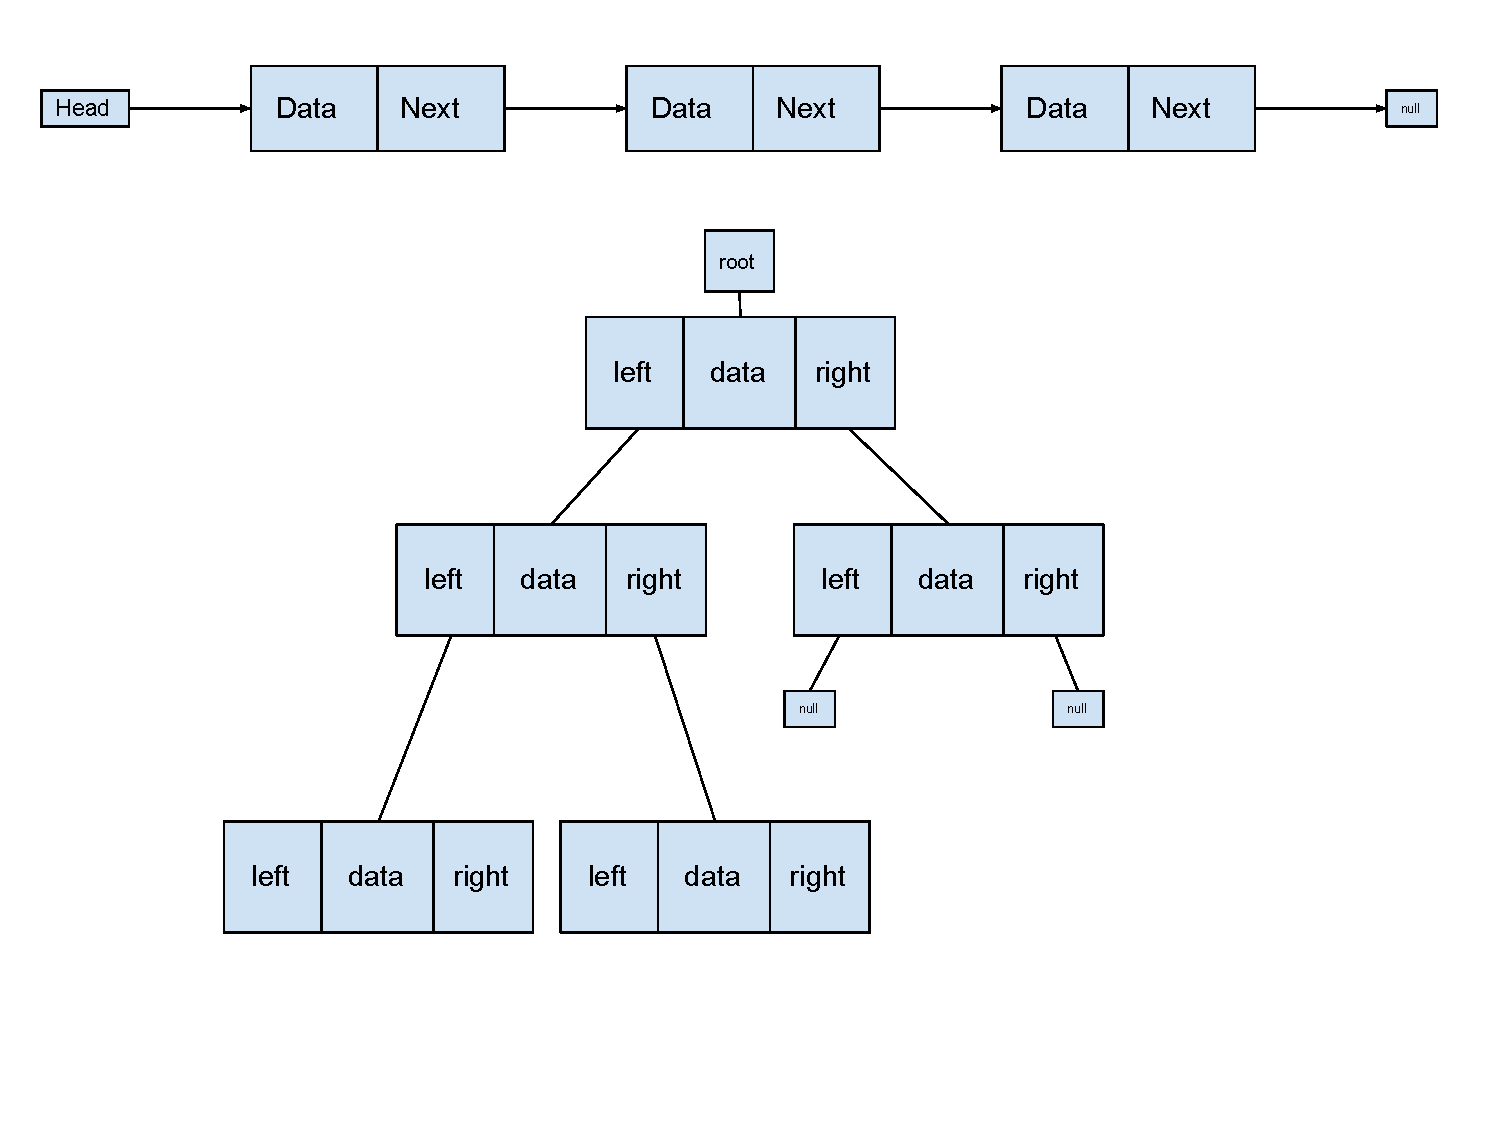
\includegraphics[width=\textwidth]{./imgs/ds.pdf}
    \end{minipage}
\end{frame}

\section{Implementing ArrayList}

\begin{frame}[fragile]
    \frametitle{Structure of ArrayList}
        \begin{lstlisting}[basicstyle=\small]
class ArrayList<E> implements List<E>{
  private static final INITIAL_SIZE = 10;
  private Object[] stuffList;
  int size;

  ArrayList(){
    stuffList = new Object[INITIAL_SIZE];
    size = 0;
  }

  public void add(E e){/*our implementation here*/}

  public boolean remove(E e){/*our implementation here*/}
}
        \end{lstlisting}
\end{frame}


\begin{frame}[fragile]
    \frametitle{Adding}
    \begin{figure}
        \centering
        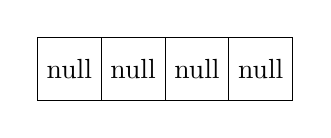
\begin{tikzpicture}
        \matrix (A) [matrix of nodes, nodes={draw, minimum size=8mm},
            column sep=-\pgflinewidth]{
            null & null & null & null \\};
        \end{tikzpicture}
        \\Size = 0
    \end{figure}
    \vfill
    \begin{lstlisting}[basicstyle=\small]
    SimpleList<Integer> nums = new SimpleArrayList<>();



.
    \end{lstlisting}
\end{frame}

\begin{frame}[fragile]
    \frametitle{Adding}
    \begin{figure}
        \centering
        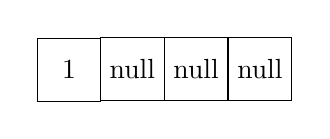
\begin{tikzpicture}
        \matrix (A) [matrix of nodes, nodes={draw, minimum size=8mm},
            column sep=-\pgflinewidth]{
            1 & null & null & null \\};
        \end{tikzpicture}
        \\Size = 1
    \end{figure}
    \vfill
    \begin{lstlisting}[basicstyle=\small]
    SimpleList<Integer> nums = new SimpleArrayList<>();
    nums.add(1);


.
    \end{lstlisting}
\end{frame}

\begin{frame}[fragile]
    \frametitle{Adding}
    \begin{figure}
        \centering
        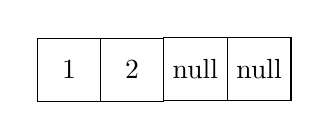
\begin{tikzpicture}
        \matrix (A) [matrix of nodes, nodes={draw, minimum size=8mm},
            column sep=-\pgflinewidth]{
            1 & 2 & null & null \\};
        \end{tikzpicture}
        \\Size = 2
    \end{figure}
    \vfill
    \begin{lstlisting}[basicstyle=\small]
    SimpleList<Integer> nums = new SimpleArrayList<>();
    nums.add(1);
    nums.add(2);

.
    \end{lstlisting}
\end{frame}

\begin{frame}[fragile]
    \frametitle{Adding}
    \begin{figure}
        \centering
        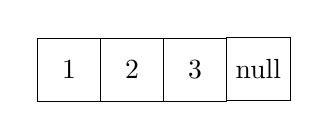
\begin{tikzpicture}
        \matrix (A) [matrix of nodes, nodes={draw, minimum size=8mm},
            column sep=-\pgflinewidth]{
            1 & 2 & 3 & null \\};
        \end{tikzpicture}
        \\Size = 3
    \end{figure}
    \vfill
    \begin{lstlisting}[basicstyle=\small]
    SimpleList<Integer> nums = new SimpleArrayList<>();
    nums.add(1);
    nums.add(2);
    nums.add(3);
.
    \end{lstlisting}
\end{frame}

\begin{frame}[fragile]
    \frametitle{Adding}
    \begin{figure}
        \centering
        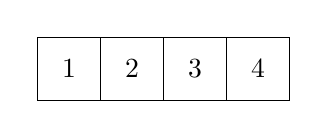
\begin{tikzpicture}
        \matrix (A) [matrix of nodes, nodes={draw, minimum size=8mm},
            column sep=-\pgflinewidth]{
            1 & 2 & 3 & 4 \\};
        \end{tikzpicture}
        \\Size = 4
    \end{figure}
    \vfill
    \begin{lstlisting}[basicstyle=\small]
    SimpleList<Integer> nums = new SimpleArrayList<>();
    nums.add(1);
    nums.add(2);
    nums.add(3);
    nums.add(4);
    //What happens when we add another element?
    \end{lstlisting}
\end{frame}

\begin{frame}[fragile]
    \frametitle{Adding}
    \begin{figure}
        \centering
        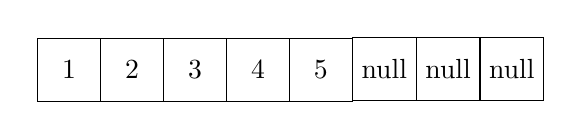
\begin{tikzpicture}
        \matrix (A) [matrix of nodes, nodes={draw, minimum size=8mm},
            column sep=-\pgflinewidth]{
            1 & 2 & 3 & 4 & 5 & null & null & null\\};
        \end{tikzpicture}
        \\Size = 5
    \end{figure}
    \vfill
    \begin{lstlisting}[basicstyle=\small]
    SimpleList<Integer> nums = new SimpleArrayList<>();
    nums.add(1);
    nums.add(2);
    nums.add(3);
    nums.add(4);
    //What happens when we add another element?
    nums.add(5);
    \end{lstlisting}
\end{frame}

\begin{frame}[fragile]
    \frametitle{Adding Method: Psudeocode}
    \begin{figure}
    \centering
    \begin{lstlisting}[basicstyle=\small]
Add(NewElement)
    EnsureCapacity(size + 1)
    List[size] = NewElement
    Size++
EndAdd
    \end{lstlisting}
    \end{figure}
\end{frame}


\begin{frame}[fragile]
    \frametitle{Ensure Capacity}
    \begin{figure}
    \centering
    \begin{lstlisting}[basicstyle=\small]
EnsureCapacity(MinSize)
    If(A.length < MinSize)
        A= CopyList(A, Size + AmountToIncreaseBy)
    EndIf
EndAdd
    \end{lstlisting}
\end{figure}
\end{frame}

\begin{frame}[fragile]
    \frametitle{Removing}
    \textbf{Condition \#1: The Item we're removing is at the end (\textcolor{green}{Good})}
    \begin{figure}[H]
        \centering
        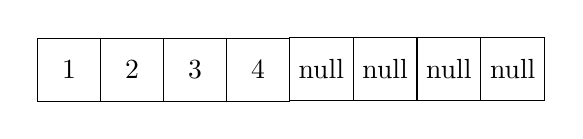
\begin{tikzpicture}
        \matrix (A) [matrix of nodes, nodes={draw, minimum size=8mm},
            column sep=-\pgflinewidth]{
            1 & 2 & 3 & 4 & null & null & null & null\\};
        \end{tikzpicture}\\
        size = 4
    \end{figure}
    \vfill
    \begin{lstlisting}[frame=trBL, basicstyle=\small]
primes[4] = null;
size = size - 1
    \end{lstlisting}
    \textbf{Condition \#2: The item is in the middle or front of the list (\textcolor{red}{Bad})} 
    \begin{figure}[H]
        \centering
        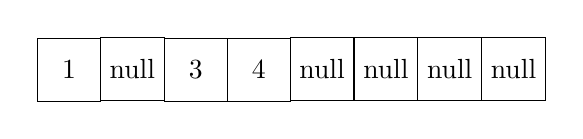
\begin{tikzpicture}
        \matrix (A) [matrix of nodes, nodes={draw, minimum size=8mm},
            column sep=-\pgflinewidth]{
            1 & null & 3 & 4 & null & null & null & null\\};
        \end{tikzpicture}\\
        size = 3 
    \end{figure}
    \vfill
    \begin{lstlisting}[frame=trBL, basicstyle=\small]
primes[1] = null;
size = size - 1
    \end{lstlisting}
\end{frame}

\begin{frame}[fragile]
    \frametitle{Why removing that way is bad}
    \begin{figure}
        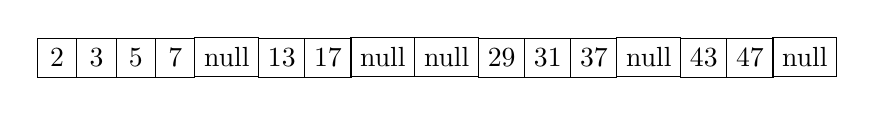
\begin{tikzpicture}
        \matrix (A) [matrix of nodes, nodes={draw, minimum size=5mm},
            column sep=-\pgflinewidth]{
            2 & 3 & 5 & 7 & null & 13 & 17 & null & null & 29 & 31 & 37 & null & 43 & 47 & null\\};
        \end{tikzpicture}
    \end{figure}
    \begin{enumerate}
        \item We can't use \lstinline|Size| to find the true end of our list.
        \item We have all these empty spaces.
        \item Where do we insert?
    \end{enumerate}
\end{frame}

\begin{frame}[fragile]
    \frametitle{How to remove \lstinline|2?|}
    \textbf{Before}:
    \begin{figure}[H]
        \centering
        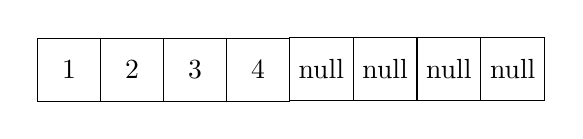
\begin{tikzpicture}
        \matrix (A) [matrix of nodes, nodes={draw, minimum size=8mm},
            column sep=-\pgflinewidth]{
            1 & 2 & 3 & 4 & null & null & null & null\\};
        \end{tikzpicture}\\
        size = 4
    \end{figure}
    \textbf{After}:
    \begin{figure}[H]
        \centering
        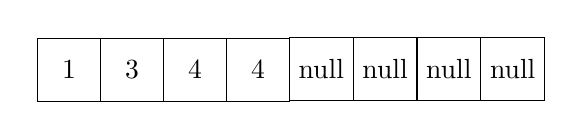
\begin{tikzpicture}
        \matrix (A) [matrix of nodes, nodes={draw, minimum size=8mm},
            column sep=-\pgflinewidth]{
            1 & 3 & 4 & 4 & null & null & null & null\\};
        \end{tikzpicture}\\
        size = 4
    \end{figure}
    \textbf{Step 1:} Copy each element to the right of the element we want to remove 1 step to the left
\end{frame}

\begin{frame}[fragile]
    \frametitle{How to remove 2?}
    \textbf{Before}:
    \begin{figure}[H]
        \centering
        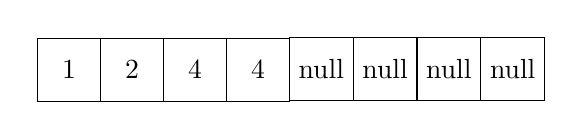
\begin{tikzpicture}
        \matrix (A) [matrix of nodes, nodes={draw, minimum size=8mm},
            column sep=-\pgflinewidth]{
            1 & 2 & 4 & 4 & null & null & null & null\\};
        \end{tikzpicture}\\
        size = 4
    \end{figure}
    \textbf{After}:
    \begin{figure}[H]
        \centering
        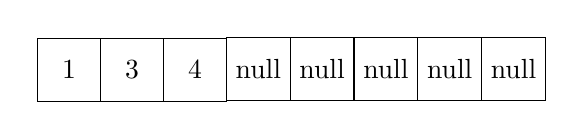
\begin{tikzpicture}
        \matrix (A) [matrix of nodes, nodes={draw, minimum size=8mm},
            column sep=-\pgflinewidth]{
            1 & 3 & 4 & null & null & null & null & null\\};
        \end{tikzpicture}\\
        size = 4
    \end{figure}
    \textbf{Step 2:} Set end of the list (element at size - 1) to \lstinline|null|.
\end{frame}

\begin{frame}[fragile]
    \frametitle{How to remove 2?}
    \textbf{Before}:
    \begin{figure}[H]
        \centering
        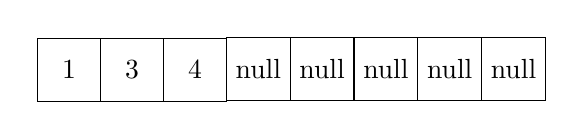
\begin{tikzpicture}
        \matrix (A) [matrix of nodes, nodes={draw, minimum size=8mm},
            column sep=-\pgflinewidth]{
            1 & 3 & 4 & null & null & null & null & null\\};
        \end{tikzpicture}\\
        size = 4
    \end{figure}
    \textbf{After}:
    \begin{figure}[H]
        \centering
        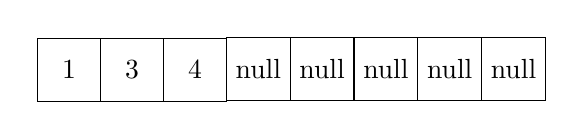
\begin{tikzpicture}
        \matrix (A) [matrix of nodes, nodes={draw, minimum size=8mm},
            column sep=-\pgflinewidth]{
            1 & 3 & 4 & null & null & null & null & null\\};
        \end{tikzpicture}\\
        size = 3 
    \end{figure}
    \textbf{Step 3:} Decrement size.
\end{frame}

\begin{frame}[fragile]
    \frametitle{Remove Method: Basic Psudeocode}
    \begin{lstlisting}[basicstyle=\small]
Remove(ElementForRemoval)
    i = Find(ElementForRemoval)

    If(ElementForRemoval not in List) 
        Return False
    EndIf
    
    If(i == Size - 1)
        // Remove from the end
    Else
        // Remove from the middle
    EndIf

    Size = Size - 1
    Return True
EndAdd
    \end{lstlisting}
\end{frame}

\begin{frame}[fragile]
    \frametitle{This Week}
    \begin{enumerate}
        \item This week you will be building a generic list interface and a generic list class that implements that interface.
        \item Some videos are up, more to come.
    \end{enumerate}
\end{frame}

\end{document}
